% Created 2024-11-05 Tue 08:31
% Intended LaTeX compiler: lualatex
\documentclass[presentation,professionalfonts,aspectratio=169]{beamer}
                

% 
\makeatletter
 \@ifclassloaded{beamer}{%
  %%% save beamer's `solution' environment as `beamersolution':
  \let\beamersolution\solution
  \let\endbeamersolution\endsolution
  %%% "delete" the `solution' environment:
  \let\solution\relax
  \let\endsolution\relax
}{%
}%
\makeatother
\usepackage[utf8]{inputenc}
\usepackage[T1]{fontenc}
%\usepackage[french]{babel}
\usepackage[portuguese]{babel}

%%%% FONTS




\usepackage{xsim}
\usepackage[most]{tcolorbox}
\usepackage{amssymb}
\usepackage{fontawesome}
\newcounter{paragraph}



\DeclareExerciseEnvironmentTemplate{custom}{%
  \begin{tcolorbox}[boxrule = 0pt]
  \tcbox[on line,colback=teal,colframe=teal,coltext=white,size=small]{%
    \faBook\sffamily\bfseries\
    \XSIMmixedcase{\GetExerciseName}
    \GetExerciseProperty{counter}%
  }\quad
}{\end{tcolorbox}}


\DeclareExerciseEnvironmentTemplate{custom2}{%
  \begin{tcolorbox}[boxrule = 0pt]
  \tcbox[on line,colback=violet,colframe=violet,coltext=white,size=small]{%
    \faToggleOn\sffamily\bfseries\
    \XSIMmixedcase{\GetExerciseName}
    \GetExerciseProperty{counter}%
  }\quad
}{\end{tcolorbox}}




\DeclareExerciseType{test}{
	exercise-env = question ,
	solution-env = answer ,
	exercise-template = custom ,
	solution-template = custom2 ,
	exercise-name	= Exemplo. ,
	exercises-name = Exemplo ,
	solution-name = Solução ,
	solutions-name = Sol. ,
	exercise-heading = \textbf ,
	solution-heading = \textbf
}


\xsimsetup{
  exercise/within = section,
  exercise/the-counter =  \arabic{exercise}, 
%%solution-name = solution,  % used with headings=true
solution/print=false,
%print-collection/print=both,
}





\usepackage{colortbl}
\usepackage[tikz]{bclogo}
\usetikzlibrary{fit,patterns,shadows.blur,shapes,mindmap}
\usetikzlibrary{arrows,calc,arrows.meta,decorations.markings,shapes.symbols}
\usetikzlibrary{decorations.pathreplacing, decorations.pathmorphing,calc,arrows,positioning}
\usepackage{tikzpeople}
\usepackage{qrcode,hyperref}
\usepackage{upgreek}
%\usepackage[version=4]{mhchem}
\usepackage{tabularray}


\NewTblrTheme{fancy}{
\SetTblrStyle{caption-tag}{font=\bfseries}
\SetTblrInner[tblr,longtblr]{rowsep=2.5pt}
\DefTblrTemplate{firsthead, middlehead,lasthead}{default}{} % <---
\DefTblrTemplate{contfoot-text}{normal}{\scriptsize\textit{Continued on the next page}}
\SetTblrTemplate{contfoot-text}{normal}
}






\usepackage{chemfig,chemmacros,elements,chemformula}
\chemsetup{modules={all}}
\chemsetup[redox]{pos=top,roman=false}
\chemsetup[redox]{pos=top}
\chemsetup{redox/sep=.5em}
\chemsetup[redox]{explicit-sign=true}
\NewChemPhase\lqdd{\(\ell\)}
\NewChemPhase\gr{grafite}
\NewChemPhase\reac{reação}
\NewChemState\Enthalpy{symbol=H,superscript=,unit=\kilo\joule}%
\usepackage{siunitx}
\setchemfig{fixed length=false, atom sep=2.5em, arrow offset=6pt, scheme debug=false}%,angle increment=30}
\renewcommand*\printatom[1]{\ensuremath{\mathsf{#1}}} % This line changes the font of the atoms to sans serif
%%%% QRCODE
\usepackage{pdfpages}
\usepackage{mol2chemfig}
\usepackage{subfig,caption}
\usepackage{wrapfig}
\usepackage{enumitem}
\setitemize{label=\usebeamerfont*{itemize item}%
\usebeamercolor[fg]{itemize item}
\usebeamertemplate {itemize item}}
\usepackage{array} % ajust colunm table
\usepackage{cancel}
\usepackage[controls]{animate}
\renewcommand{\CancelColor}{\color{red}}

%%%%%%%%%%%%%%%%%%% CONFIG TCOLORBOX 

\newtcolorbox{mybox}[2][]{boxsep=0.5em,left=0.5em,
colback=blue!5!white, colframe=blue!75!black,
fonttitle=\bfseries\sffamily,
colbacktitle=blue!85!red!60,enhanced,
attach boxed title to top left={yshift=-3mm,xshift=5mm},
title=#2,#1}

\newtcolorbox{myrule}[2][]{boxsep=0.5em,left=0.5em,
colback=green!5!white, colframe=blue!75!black,
fonttitle=\bfseries\sffamily,
colbacktitle=blue!85!red!60,enhanced,
attach boxed title to top left={yshift=-3mm,xshift=5mm},
title=#2,#1}


\newtcolorbox{myex}[2][]{boxsep=0.5em,left=0.5em,
  colback=yellow!5!white, colframe=blue!75!black, 
  fonttitle=\bfseries\sffamily,
  colbacktitle=blue!85!red!60,enhanced,
  attach boxed title to top left={yshift=-3mm,xshift=5mm},
  title=#2,#1}


 \definecolor{col1}{HTML}{FF7878}
 \definecolor{col2}{HTML}{51B5F8}
 \definecolor{col3}{HTML}{68E1AA}
 \definecolor{col4}{HTML}{B869EA}
 \definecolor{col5}{HTML}{FF5500}
 \definecolor{col6}{HTML}{FFF8E7}
 \definecolor{col7}{HTML}{FF9966}
 \definecolor{col8}{HTML}{9400D3}



\definesubmol\nobond{-[,0.2,,,draw=none]\scriptstyle\color{blue}}
\newcommand{\re}{\hspace{-1cm}}
\newcommand{\af}{\hspace{2cm}}

%%%% Config X sim for BEAMER
\usepackage{ragged2e}
\justifying
\makeatletter
\@ifclassloaded{beamer}{%
%%% save beamer's `solution' environment as `beamersolution':
\let\beamersolution\solution
\let\endbeamersolution\endsolution
%%% "delete" the `solution' environment:
\let\solution\relax
\let\endsolution\relax
}{%
}%
\makeatother
\usepackage[utf8]{inputenc}
\usepackage[T1]{fontenc}
%\usepackage[portuguese, ]{babel}
%%%% FONTS
%%% XSIM CONFIG BEAMER
\usepackage{xsim}
\usepackage{amsmath}
\usepackage[most]{tcolorbox}
\usepackage{amssymb}
\usepackage{fontawesome}
\usepackage{tasks}
\newcounter{paragraph}
%\usepackage[dvipsnames,svgnames]{xcolor}
\usepackage{xcolor}
\usepackage{annotate-equations}
%%% BOX EXERCISE BEAMER
\DeclareExerciseEnvironmentTemplate{custom}{%
\begin{tcolorbox}[boxrule = 0pt]
\tcbox[on line,colback=teal,colframe=teal,coltext=white,size=small]{%
\faBook\sffamily\bfseries\
\XSIMmixedcase{\GetExerciseName}
\GetExerciseProperty{counter}%
}\quad
}{\end{tcolorbox}}
%% == CUSTOM BOX BEAMER
\DeclareExerciseEnvironmentTemplate{custom2}{%
\begin{tcolorbox}[boxrule = 0pt]
\tcbox[on line,colback=violet,colframe=violet,coltext=white,size=small]{%
\faToggleOn\sffamily\bfseries\
\XSIMmixedcase{\GetExerciseName}
\GetExerciseProperty{counter}%
}\quad
}{\end{tcolorbox}}
\DeclareExerciseType{test}{
exercise-env = question ,
solution-env = answer ,
exercise-template = custom ,
solution-template = custom2 ,
exercise-name = Exemplo ,
exercises-name = Exemplo ,
solution-name = Solução ,
solutions-name = Sol. ,
exercise-heading = \textbf ,
solution-heading = \textbf
}
\xsimsetup{
exercise/within = section,
exercise/the-counter =  \arabic{exercise},
%%solution-name = solution,  % used with headings=true
solution/print=true,
print-collection/print=both,
}
\NewTasksEnvironment[label = (\emph{\alph*}),
label-width = 12pt]{choice}[\choice]
\usepackage{empheq} %%% Brackers
\usepackage{colortbl}
\usepackage[tikz]{bclogo}
\usetikzlibrary{fit,patterns,shadows.blur,shapes,mindmap}
\usetikzlibrary{arrows,arrows.meta,decorations.markings,shapes.symbols}
\usetikzlibrary{decorations.pathreplacing, decorations.pathmorphing,calc,arrows,positioning,snakes}
\usepackage{tikzpeople}
\usepackage{qrcode,hyperref}
\usepackage{upgreek}
%\usepackage[version=4]{mhchem}
\usepackage{tabularray}
%%% PACKAGE PLOT GRAPH
\usepackage{pgfplots}
\pgfplotsset{width=10cm,compat=1.9}
%%% CUSTOM TABLE
\NewTblrTheme{fancy}{
\SetTblrStyle{caption-tag}{font=\bfseries,red2}
\SetTblrInner[tblr,longtblr]{rowsep=2.5pt}
\DefTblrTemplate{firsthead, middlehead,lasthead}{default}{} % <---
\DefTblrTemplate{contfoot-text}{normal}{\scriptsize\textit{Continua ...}}
\SetTblrTemplate{contfoot-text}{normal}
}
%% ==== CHEMMACROS E CHEMFIG CONFIG
\usepackage{chemfig,chemmacros,elements,chemformula}
\chemsetup{modules={all}}
\chemsetup[redox]{pos=top,roman=false}
\chemsetup[redox]{pos=top}
\chemsetup{redox/sep=.5em}
\chemsetup[redox]{explicit-sign=true} %%% reaction redox
%% == CUSTOM PHASES IN CHEMMACROS
\NewChemPhase\lqdd{\(\ell\)}
\NewChemPhase\gr{grafite}
\NewChemPhase\reac{reação}
\NewChemState\Enthalpy{symbol=H,superscript=,unit=\kilo\joule}%
\usepackage{siunitx}
\setchemfig{fixed length=false, atom sep=2.5em, arrow offset=6pt, scheme debug=false}
%% == NUMEROS PARA FORMULES
\renewcommand*\printatom[1]{\ensuremath{\mathsf{#1}}} % This line changes the font of the atoms to sans serif
%%% INCLUDE PAGES PDFs
\usepackage{pdfpages}
\usepackage{mol2chemfig}
\usepackage{xymtexpdf}
\changeunitlength{0.08pt}
\usepackage{subfig,caption}
\usepackage{wrapfig}
\usepackage{enumitem}
\setitemize{label=\usebeamerfont*{itemize item}%
\usebeamercolor[fg]{itemize item}
\usebeamertemplate {itemize item}}
\usepackage{array} % ajust colunm table
\usepackage{cancel}
\usepackage[controls]{animate}
\renewcommand{\CancelColor}{\color{red}}
%%%%%%%%%%%%%%%%%%% CONFIG TCOLORBOX
\newtcolorbox{mybox}[2][]{boxsep=0.5em,left=0.5em,
colback=blue!5!white, colframe=blue!75!black,
fonttitle=\bfseries\sffamily,
colbacktitle=blue!85!red!60,enhanced,
attach boxed title to top left={yshift=-3mm,xshift=5mm},
title=#2,#1}
\newtcolorbox{myrule}[2][]{boxsep=0.5em,left=0.5em,
colback=green!5!white, colframe=blue!75!black,
fonttitle=\bfseries\sffamily,
colbacktitle=blue!85!red!60,enhanced,
attach boxed title to top left={yshift=-3mm,xshift=5mm},
title=#2,#1}
\newtcolorbox{myex}[2][]{boxsep=0.5em,left=0.5em,
colback=yellow!5!white, colframe=blue!75!black,
fonttitle=\bfseries\sffamily,
colbacktitle=blue!85!red!60,enhanced,
attach boxed title to top left={yshift=-3mm,xshift=5mm},
title=#2,#1}
\tcbset{colback=yellow!10!white, colframe=red!50!black, highlight math style= {enhanced, %<-- needed for the ’remember’ options
colframe=red,colback=red!10!white,boxsep=0pt}}
\definecolor{col1}{HTML}{FF7878}
\definecolor{col2}{HTML}{51B5F8}
\definecolor{col3}{HTML}{68E1AA}
\definecolor{col4}{HTML}{B869EA}
\definecolor{col5}{HTML}{FF5500}
\definecolor{col6}{HTML}{FFF8E7}
\definecolor{col7}{HTML}{FF9966}
\definecolor{col8}{HTML}{9400D3}
%% CONFIG COLOR CARBONO
\tikzstyle{bal}=[inner sep=0.3pt,fill=orange,fill opacity=0.5,circle,minimum size=0.2cm]
\tikzstyle{rect}=[inner sep=0.3pt,fill=red,fill opacity=0.5,circle,minimum size=0.2cm]
\tikzstyle{bal2}=[inner sep=0.3pt,fill=blue,fill opacity=0.5,circle,minimum size=0.2cm]
\tikzstyle{bal3}=[inner sep=0.3pt,fill=yellow,fill opacity=0.5,circle,minimum size=0.2cm]
\definesubmol\nobond{-[,0.2,,,draw=none]\scriptstyle\color{blue}}
\newcommand{\re}{\hspace{-1cm}}
\newcommand{\af}{\hspace{2cm}}
\tikzstyle{mybox} = [draw=red, fill=blue!20, very thick, rectangle, rounded corners, inner sep=10pt, inner ysep=20pt]
\tikzstyle{fancytitle} =[fill=red, text=white]
\date{}
%\usetheme{minflat}
\usetheme{minflat}
\author{Fábio Lima}
\date{}
\title{ Isomeria Geométrica}
\hypersetup{
 pdfauthor={Fábio Lima},
 pdftitle={ Isomeria Geométrica},
 pdfkeywords={},
 pdfsubject={},
 pdfcreator={Emacs 29.4 (Org mode 9.6.15)}, 
 pdflang={En Portuguese}}
\begin{document}

\maketitle
\begin{frame}{Sumário}
\tableofcontents
\end{frame}


\section{Isomeria Geométrica}
\label{sec:orgc9ec6eb}

\begin{frame}[label={sec:orgcf42248}]{Isomeria Geométrica}
\begin{itemize}
\item Conhecida como a isomeria \emph{cis-trans}.
\item Ocorre em compostos com dupla ligação ou cíclicos .
\item Compostos com dupla ligação.
\end{itemize}


\begin{columns}
\begin{column}{0.4\columnwidth}
\begin{figure}[htbp]
\centering
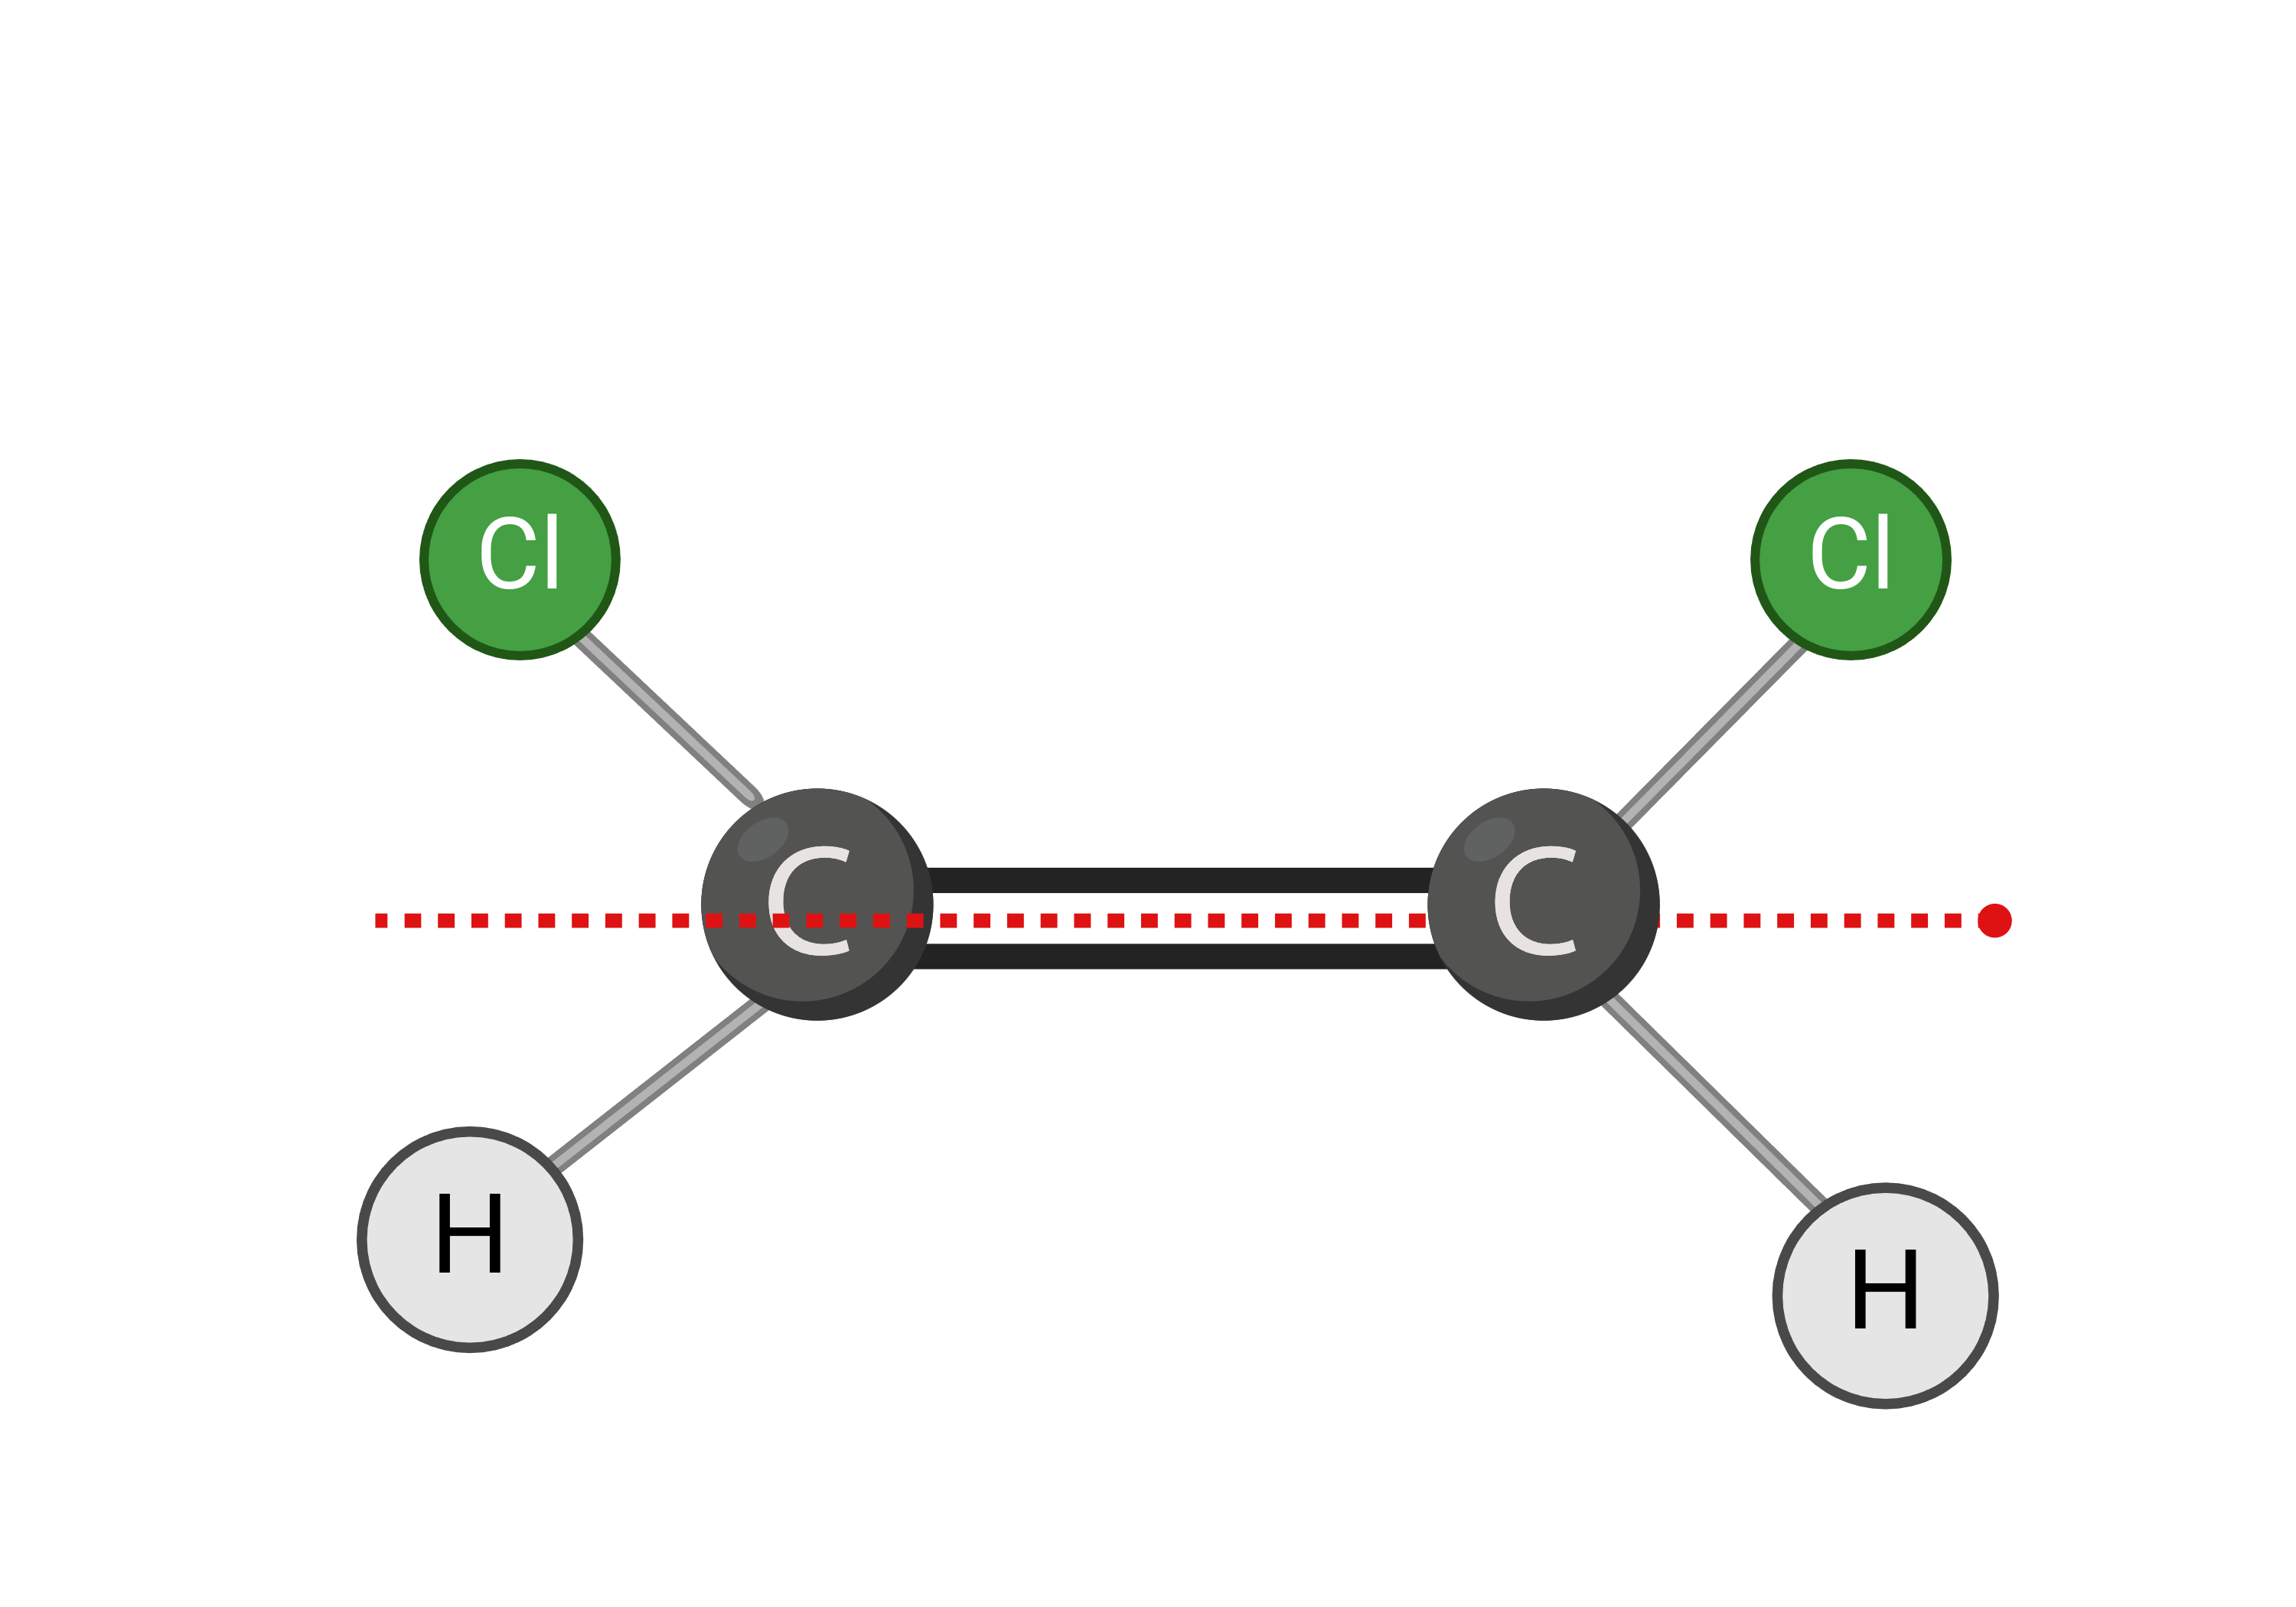
\includegraphics[width=.9\linewidth]{QO/Isomeria/CIS.png}
\caption{\emph{cis} grupos do mesmo lado. \emph{cis}-1,2-dicloro-eteno}
\end{figure}
\end{column}

\begin{column}{0.4\columnwidth}
\begin{figure}[htbp]
\centering
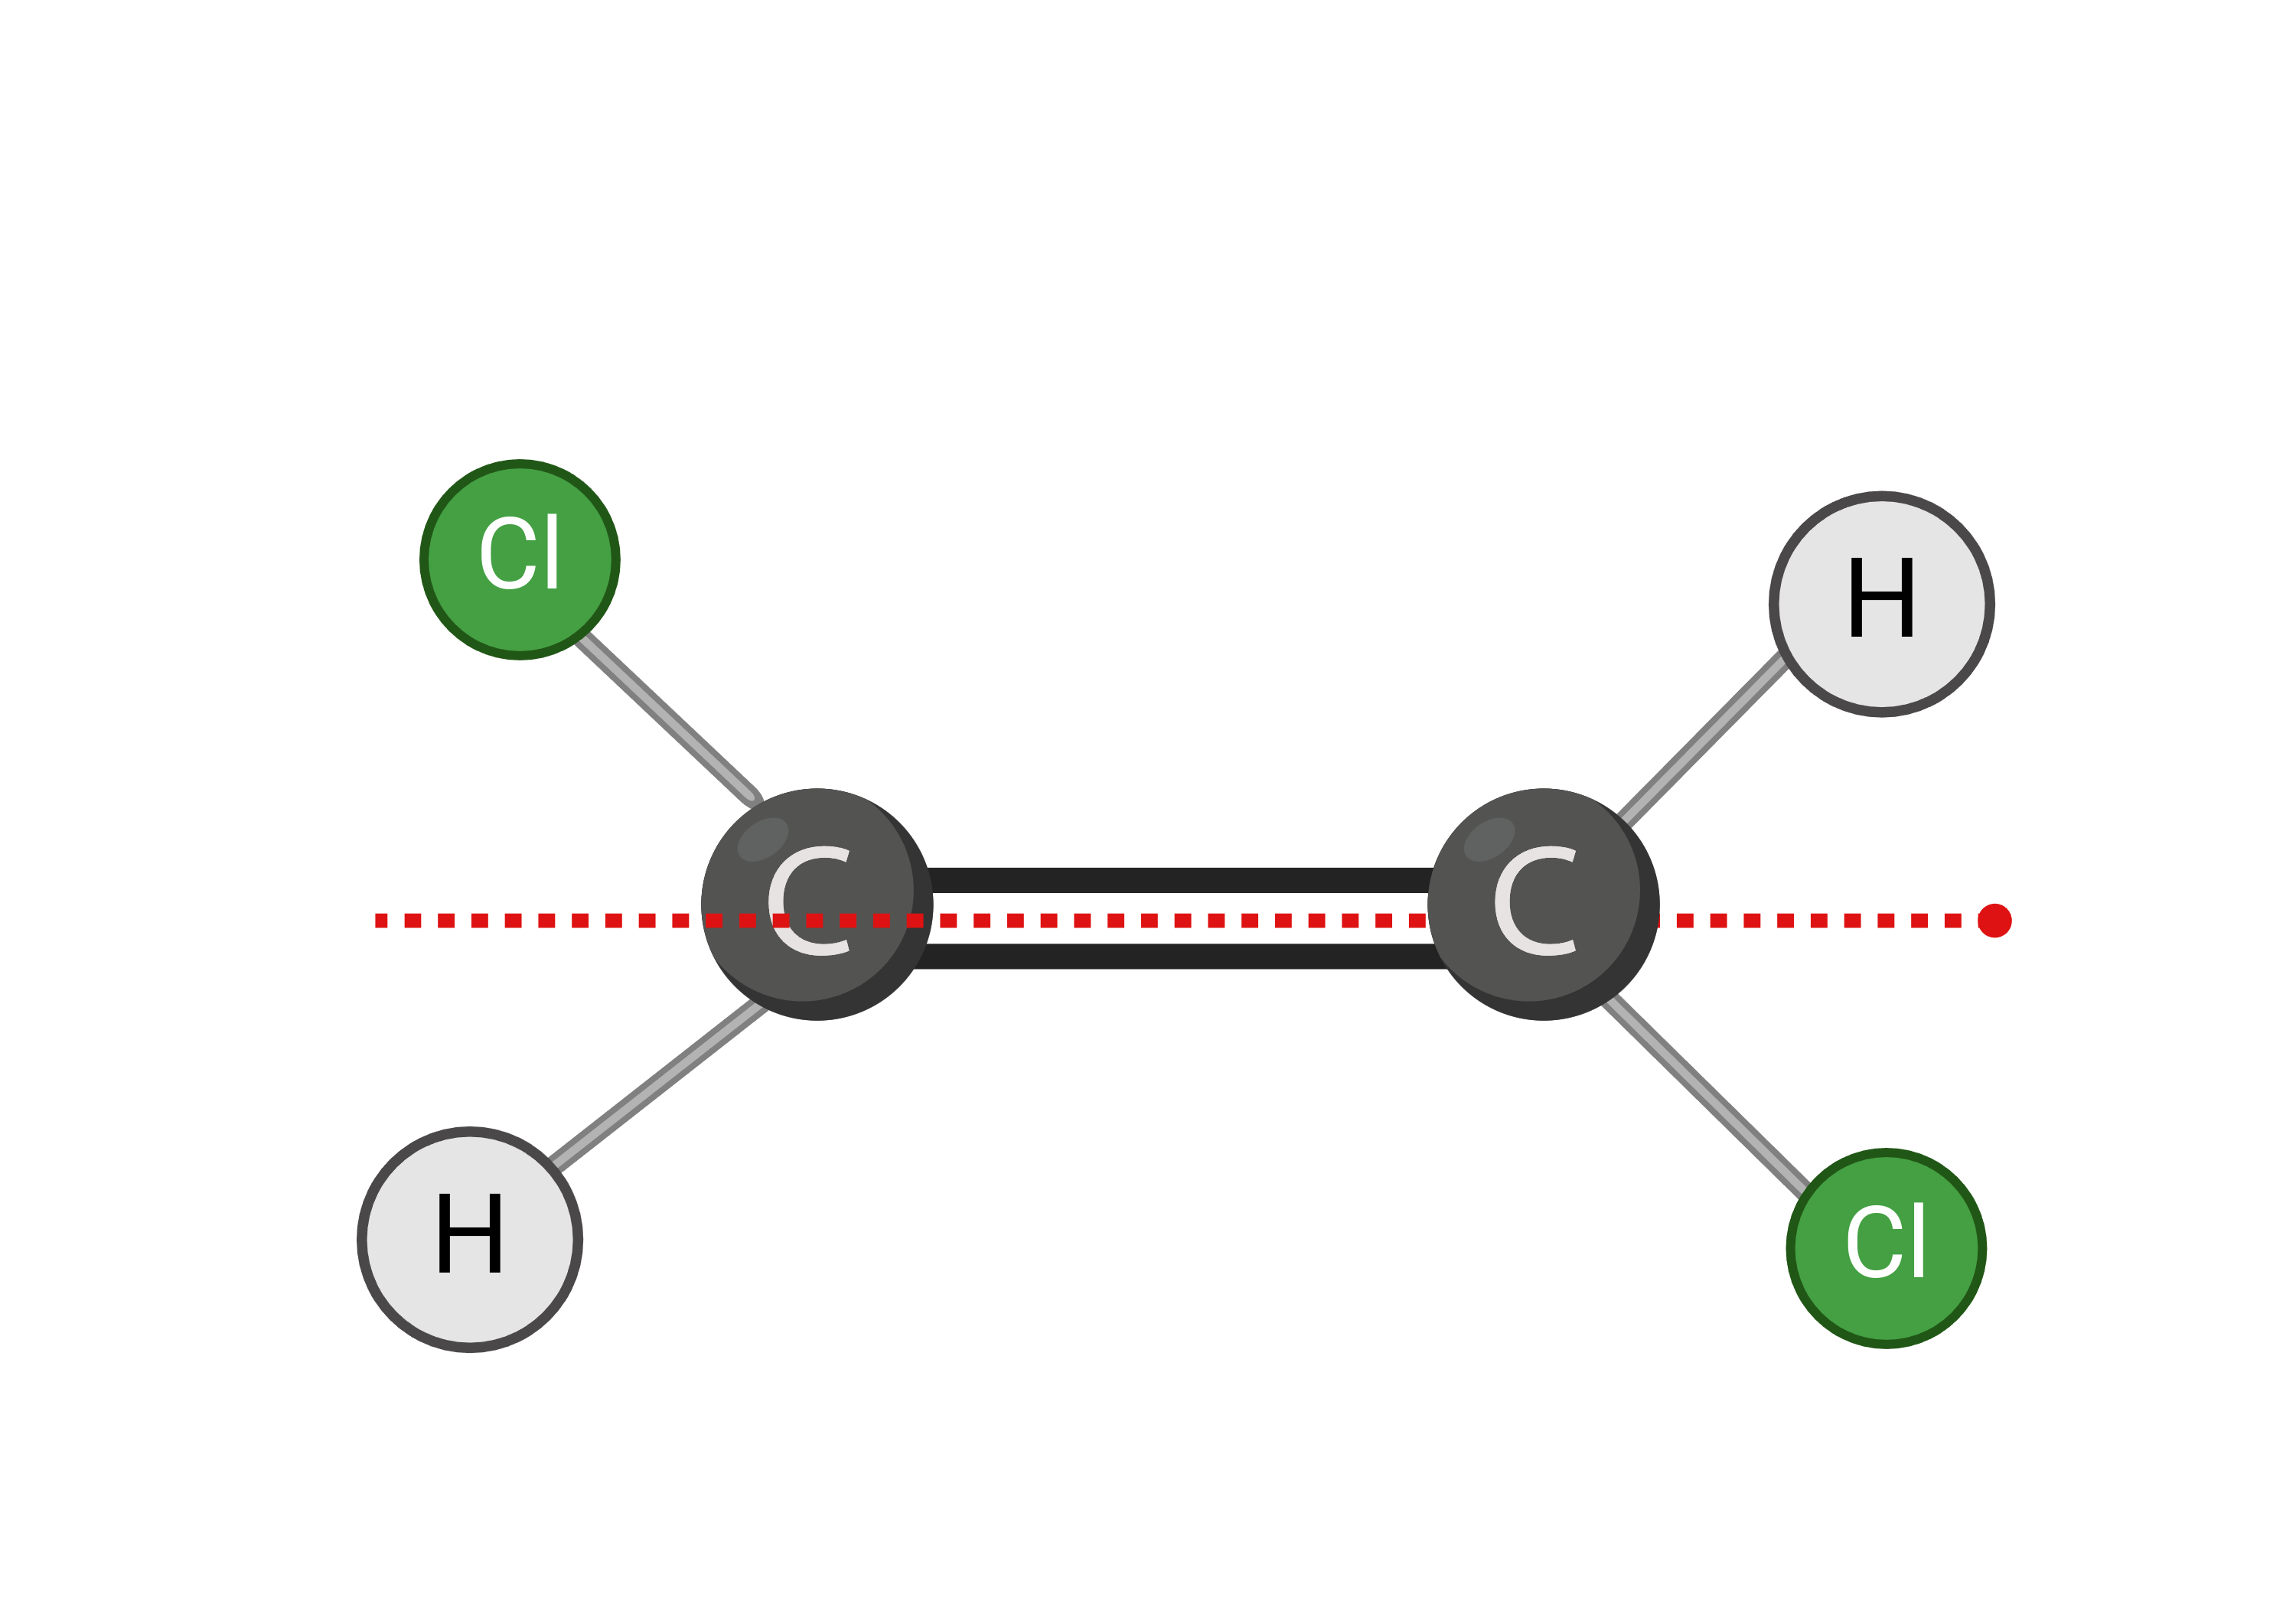
\includegraphics[width=.9\linewidth]{QO/Isomeria/Trans.png}
\caption{\emph{trans} grupos de lados opostos.  \emph{cis}-1,2-dicloro-eteno}
\end{figure}
\end{column}
\end{columns}
\end{frame}



\section{Isomeria dos  Compostos cíclicos}
\label{sec:orgbe59c15}
\begin{frame}[label={sec:org5d99ea1}]{Compostos cíclicos}
\schemestart
\chemname{\chemfig{@{a1}H_3C@{a2}>[:330,,2](<:[:225]H)-(<[:30,,,1]@{a3}CH_3@{a4})(<:[:315]H)-[:240](%
-[:120])}}{{\itshape cis}-1,2-dimetilcicloprano} 
\schemestop
\chemmove{
\node[inner sep=2pt,fill=red,fill opacity=0.2, fit=(a1) (a2)]{};
\node[inner sep=2pt,fill=red,fill opacity=0.2, fit=(a3) (a4)]{};
}
\hspace{2cm}


\schemestart
\chemname{\chemfig{@{a1}H_3C@{a2}>[:330,,2](<:[:225]H)-(<[:30]H)(<:[:315,,,1]@{a3}CH_3@{a4})-[:240](%
-[:120])}}{{\itshape trans}-1,2-dimetilcicloprano}
\schemestop
\chemmove{
    \node[inner sep=2pt,fill=red,fill opacity=0.2, fit=(a1) (a2)]{};
    \node[inner sep=2pt,fill=red,fill opacity=0.2, fit=(a3) (a4)]{};
}


\wedgehasheddash
\cyclohexanev{2B==OH;3A==OH}
\cyclohexanev{2SA==H;2SB==OH;3SA==OH;3SB==H}
\cyclohexanev{2SA==H;2SB==OH;3Sd==OH;3Su==H}
\end{frame}


\begin{frame}[label={sec:org35391bb}]{Alquenos Dissubstituídos}
\begin{itemize}
\item Os termos \emph{cis} e \emph{trans} são usados apenas para alcenos \alert{dissubstituídos}.
\end{itemize}

\begin{center}
\small
\schemestart
\chemname{\chemfig{H_3C-[:-60]C(-[:-120]H)=C(-[:-60]H)-[:60]CH_3}}{\bfseries{\itshape cis}-but-2-eno}
\qquad
\chemname{\chemfig{H-[:-60]C(-[:-120]H_3C)=C(-[:-60]H)-[:60]CH_3}}{\bfseries{\itshape trans}-but-2-eno}
\qquad
\chemname{\chemfig{H_3CCH_2-[:-60,,3]C(-[:-120]H)=C(-[:-60]H)-[:60]CH_3}}{\bfseries{\itshape cis}-pent-2-eno}
\qquad
\chemname{\chemfig{H-[:-60]C(-[:-120]H_3C)=C(-[:-60]H)-[:60]CH_2CH_3}}{\bfseries{\itshape trans}-pent-2-eno}
\schemestop
\end{center}
\end{frame}




\begin{frame}[label={sec:orga77f203}]{Exemplos}
\begin{question}
\scriptsize\{
(\alert{UERJ}) O ácido linoleico, essencial à dieta humana, apresenta a seguinte fórmula estrutural espacial:

\begin{center}
%\chemfig{-[:330]-[:30]-[:330]-[:30]-[:330]=[:30]-[:330]-[:30]=[:330]-[:30]%
%-[:330]-[:30]-[:330]-[:30]-[:330]-[:30]-[:330](=[:30]O)-[:270]H}
{\scriptsize

\chemfig{OH-[:150,,1](=[:90]O)-[:210]-[:150]-[:210]-[:150]-[:210]-[:150]%
-[:210]-[:150]=[:210]-[:270]-[:210]=[:150]-[:90]-[:150]-[:90]-[:150]-[:90]}
}
\end{center}
Como é possível observar, as ligações duplas presentes nos átomos de carbono 9 e 12 afetam o formato espacial da molécula. As conformações espaciais nessas ligações duplas são denominadas, respectivamente:

\begin{choice}(2)
\choice cis e cis
\choice cis e trans
\choice trans e cis
\choice trans e trans
\end{choice}
\}
\end{question}
\end{frame}

\begin{frame}[label={sec:org42d3a4c}]{}
\begin{answer}[print=true]
\scriptsize{
Analisando as duas insaturações das moléculas, observa-se que os ligantes não mostrados são átomos de hidrogênio. Em ambas as insaturações, os átomos de hidrogênio estão do mesmo lado da ligação dupla, logo estão em posição \alert{cis}.

\chemfig{OH-[:150,,1](=[:90]O)-[:210]-[:150]-[:210]-[:150]-[:210]-[:150]%
-[:210]-[:150](-[:90]H)=[:210](-[:150]H)-[:270]-[:210](-[:270]H)=[:150](%
-[:210]H)-[:90]-[:150]-[:90]-[:150]-[:90]}
}
\end{answer}
\end{frame}



\section{Regra de Cahn–Ingold–Prelog}
\label{sec:org5990230}
\begin{frame}[allowframebreaks]{Prefixos E e Z}
\begin{itemize}
\item Para designar alquenos tri e tetrassubstituídos utiliza-se outro sistema de nomenclatura, denominado \alert{E-Z}.
\item No sistema E-Z são examinados os grupos ligados a cada átomo de carbono da dupla ligação e colocados em ordem de prioridade.
\item Os átomos de maior número atômico têm maior prioridade. Ordem decrescente de prioridade:
\end{itemize}

\begin{center}
\schemestart
I > Br > \ch{C$\ell$} > S > F > O > N > C > H
\schemestop
	\chemmove{
	\node[single arrow, draw=black, fill=red8!30, 
	minimum width = 10pt, single arrow head extend=3pt,
	minimum height=10mm, below=1cm of c1,font=\bfseries] {Ordem descrescente de prioridade}; % length of arrow
	}
	\end{center}

\framebreak

\begin{itemize}
\item No caso de átomos de mesmo número atômico, o isótopo de maior número de massa tem maior prioridade:

\begin{tcolorbox}[colback=red!5!white,colframe=red!75!black]
 Hidrogênio \ch{->} \isotope{3,H} > \isotope{2,H} > \isotope{1,H}\\
 Carbono \ch{->} \isotope{14,C} > \isotope{13,C} > \isotope{12,C} 
\end{tcolorbox}

\item Quando os átomos ligados aos carbonos da ligação dupla forem iguais, os números e as massas atômicas dos elementos ligados a esses átomos são usados para realizar o desempate.
\item No sistema \alert{E-Z}, examinam-se os dois átomos ou grupos ligados em cada um dos carbonos da ligação dupla e determina-se a ordem de prioridade de cada um deles.
\item Se os grupos de maior prioridade em cada carbono estiverem do mesmo lado de um plano imaginário passando por esses carbonos, a geometria dessa dupla ligação será designada pela letra Z (do alemão \emph{Zusammen}, \alert{“juntos”}).
\item Se os grupos de maior prioridade em cada carbono estiverem em lados opostos da dupla ligação, a geometria da ligação será designada pela letra E (do alemão \emph{Entgegen}, \alert{“opostos”}).
\end{itemize}

\framebreak


\begin{center}
\schemestart                                           
\chemfig{@{a1}C{\ell}@{a2}-[:-60,1]C(-[:-120]@{a4}F)=C(-[:-60]@{a5}H)-[:60]@{a3}Br}
\schemestop
\end{center}

\begin{itemize}
\item Os átomos ligados ao \alert{C1} são Cl (prioridade 1) e F (prioridade 2) e os ligados ao \alert{C2}, Br (prioridade 1) e H (prioridade 2). Grupos de maior prioridade ligados do mesmo lado da dupla.
\end{itemize}

\vspace{.4cm}
\begin{center}
\schemestart                                           
\chemname[4ex]{\chemfig{@{a1}C{\ell}@{a2}-[:-60,1]C(-[:-120]@{a4}F)=C(-[:-60]@{a5}H)-[:60]@{a3}Br}}{\textcolor{red}{(Z )-2-bromo-1-cloro-1-fluoroeteno}}
\schemestop
\chemmove{
\node[circle, draw, inner sep=2pt,above=.2cm of a1] (label) {1};
\node[circle, draw, inner sep=2pt,above=.2cm of a3] (label) {1};
\node[circle, draw, inner sep=2pt,below=.2cm of a4] (label) {2};
\node[circle, draw, inner sep=2pt,below=.2cm of a5] (label) {2};
}
\end{center}


\framebreak


\begin{center}
\schemestart                                           
\chemname[6ex]{\chemfig{@{a1}H_3C@{a2}-[:-60,1]C(-[:-120]@{a4}H)=C(-[:-60]@{a5}H)-[:60]@{a3}CH_3}}{\bfseries {\itshape Z}-but-2-eno} \qquad \qquad  \qquad 
\chemname[6ex]{\chemfig{@{a7}H_3C@{a7}-[:-60,1]C(-[:-120]@{a8}H)=C(-[:-60]@{a9}CH_3)-[:60]@{a10}H}}{\bfseries {\itshape E}-but-2-eno}
\schemestop
\chemmove{
\node[circle, draw, inner sep=2pt,above=.2cm of a1] (label) {1};
\node[circle, draw, inner sep=2pt,above=.2cm of a3] (label) {1};
\node[circle, draw, inner sep=2pt,below=.2cm of a4] (label) {2};
\node[circle, draw, inner sep=2pt,below=.2cm of a5] (label) {2};
%%%%% MOLECULA 2
\node[circle, draw, inner sep=2pt,above=.33cm of a7] (label) {1};
\node[circle, draw, inner sep=2pt,above=.33cm of a10] (label) {2};
\node[circle, draw, inner sep=2pt,below=.3cm of a8] (label) {2};
\node[circle, draw, inner sep=2pt,below=.3cm of a9] (label) {1};
}

\end{center}


\framebreak

\begin{center}
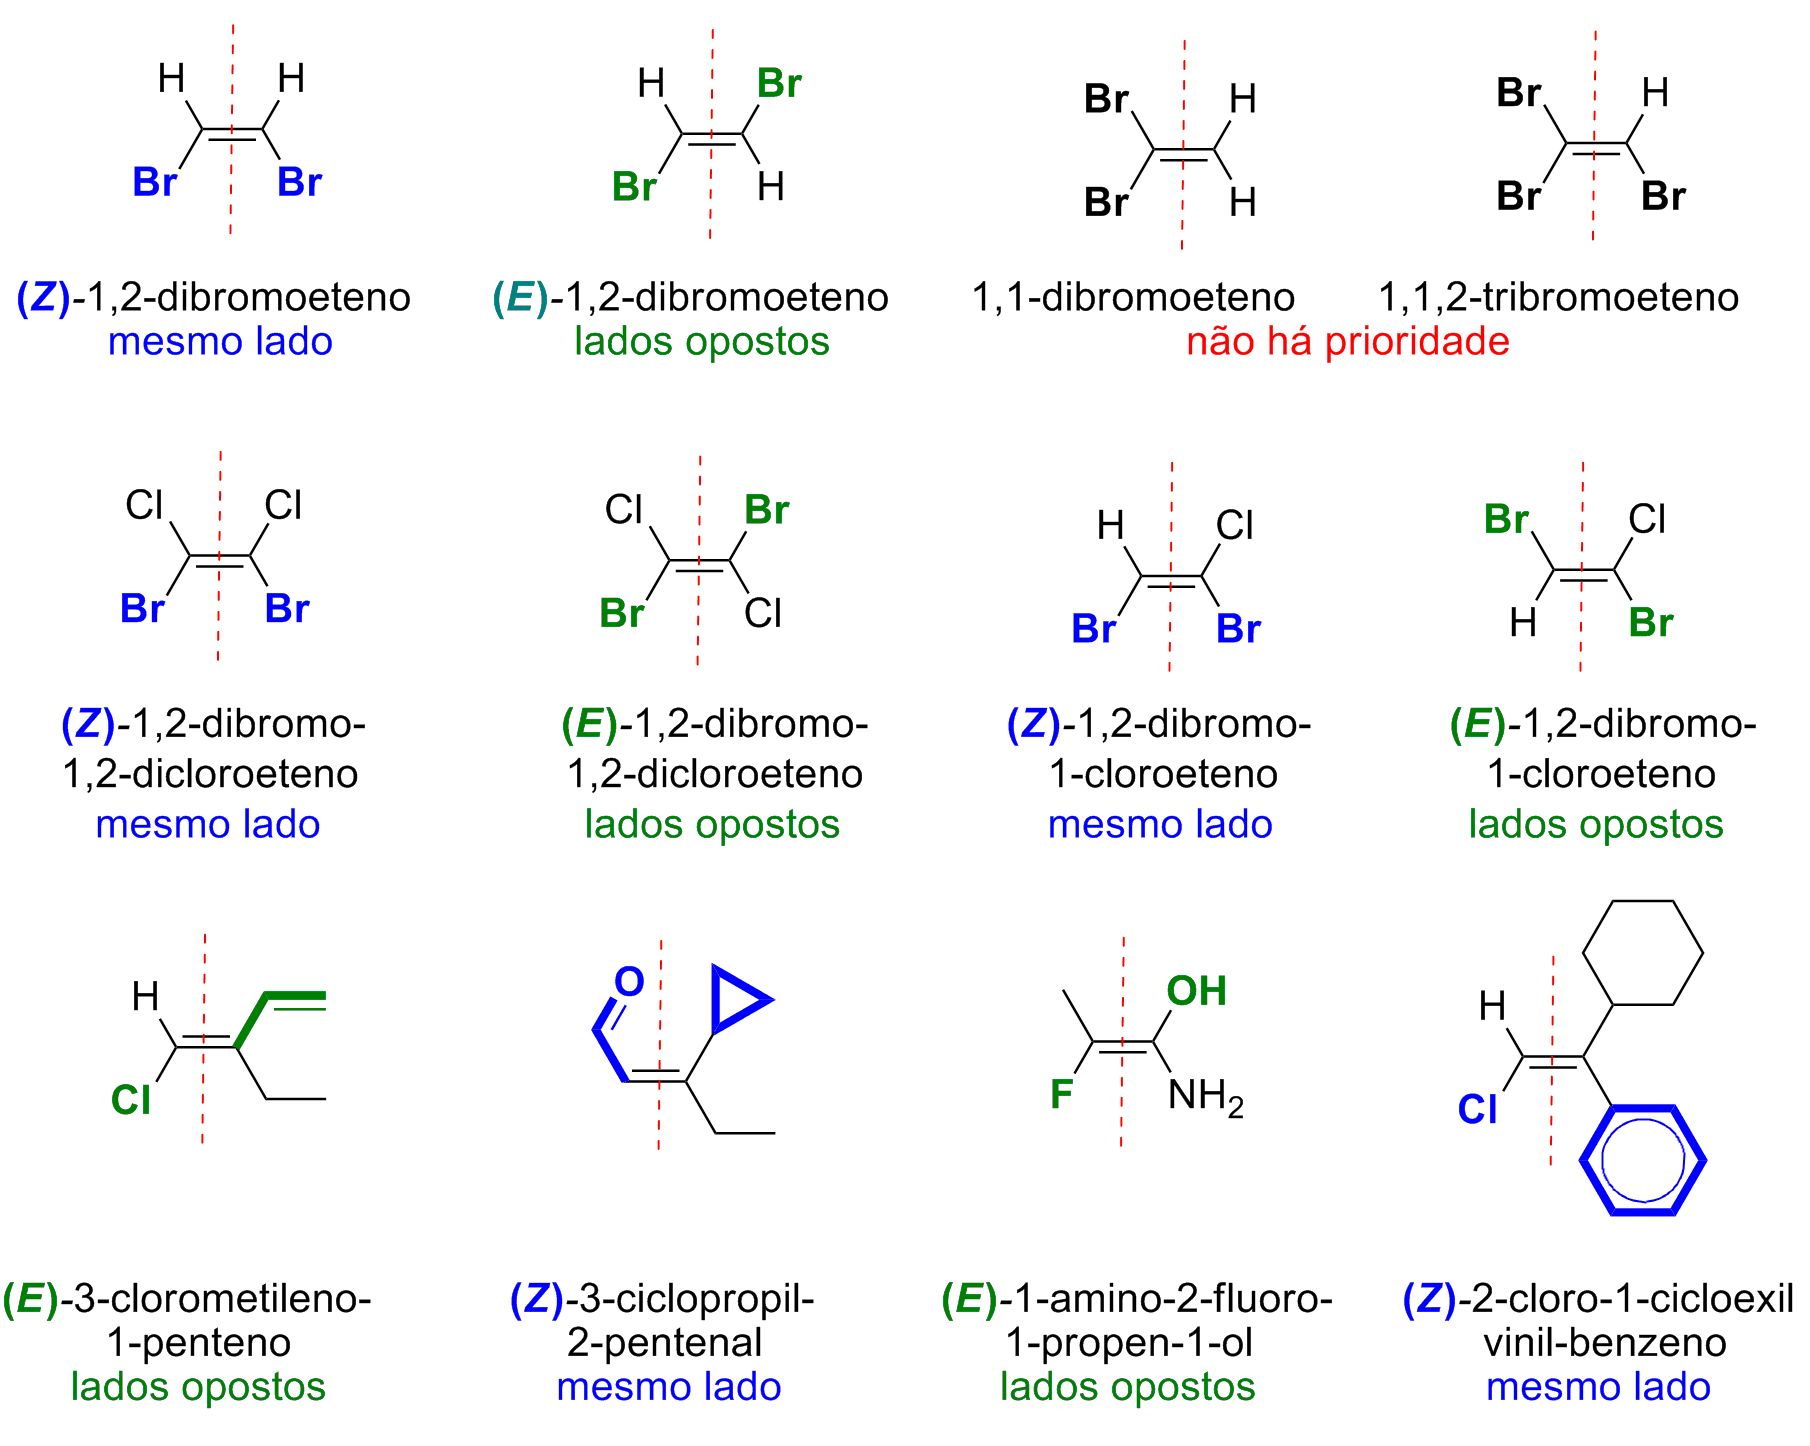
\includegraphics[scale=0.22]{QO/Isomeria/org_ez.png}
\end{center}
\end{frame}

\section{Isomeria Geométrica com Heteroátomos}
\label{sec:org101c668}

\begin{frame}[label={sec:org83b5884}]{Isomeria Geométrica com Heteroátomos}
\begin{itemize}
\item Algumas funções que contém ligados a carbono sp\textsuperscript{2}, como as oximas e iminas, possuem geometria definida já que o giro em torno da ligação \(\pi\) possui energia em geral proibitiva. Esses compostos podem ser nomeados seguindo o sistema (\alert{E})-(\alert{Z}) como utilizado em alcenos.
\end{itemize}

\begin{center}
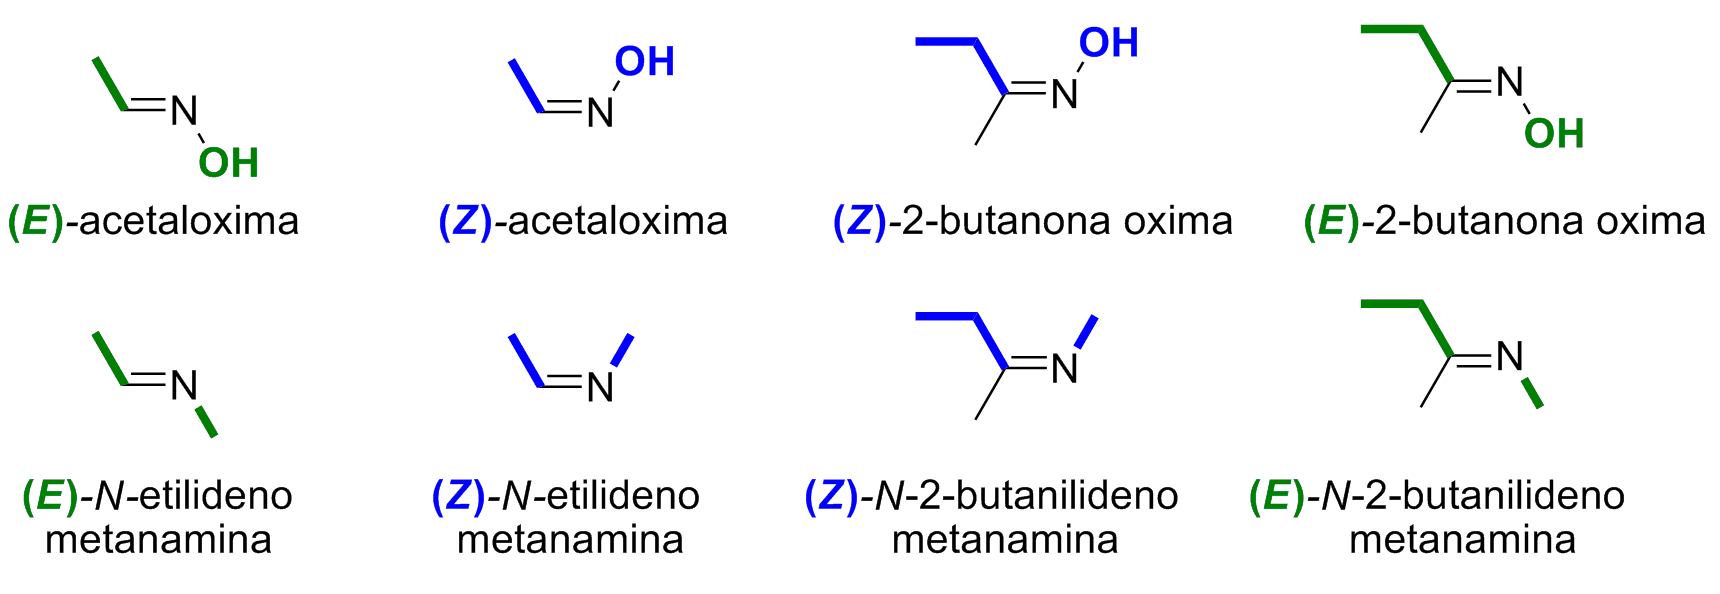
\includegraphics[width=.9\linewidth]{QO/Isomeria/org_ez_hetero.png}
\end{center}
\end{frame}







\begin{frame}[label={sec:org275a8ed}]{Fim da Aula}
\begin{tikzpicture}
\node[graduate,sword, minimum size=1cm]{ \bfseries Bons Estudos !!!!};
\end{tikzpicture}
\begin{center}
\begin{tabular}{ccc}
Download Aula  \\%& & Lista de Exercícios \\
 \qrcode[height=2in]{https://github.com/fabinholima/AulaQuimicaPDF/blob/main/QO/Isomeria/Isomeria_Geometrica.pdf} \\  %& & \qrcode[height=2in]{https://mark.nl.tab.digital/s/6kSsDYwW4icCK9X}\\
 \end{tabular}
 \end{center}
\end{frame}
\end{document}
